\documentclass[12pt]{article}

\usepackage{graphicx}
\graphicspath{{../Fichier_Image}}

\title{Hypothèse 1.(b) Taille Couloir Unique}
\author{Thibault Clodion}

\begin{document}

\maketitle % Permet d'afficher le titre, l'author etc

\underline{Hypothèse :} La taille de tous les couloirs doit être unique (pas d'effet entonnoir)
\newline\newline
\underline{Expérience :} Je pars pour cette expérience du bâtiment 10. (des 10 premiers batiments) car c'est celui ayant le meilleur temps et où les couloirs autres que le principal sont le plus emprunté.
\newline\newline
Je garde le couloir principal selon le 1.a (donc 1m) et je change la taille des autres couloirs en 80cm, 1m, 1m25, 1m50, 2m.
\newline
Une autre expérience où je change tous les couloirs : 80cm, 1m, 1m25, 1m50, 2m. (pour vérifier si l'unicité est importante)
\newline\newline

\section{Couloirs Autre}

1.(b) Couloir Autre 80cm :
\newline\newline
Temps moyen de dernière sortie : 22.67 s
\newline
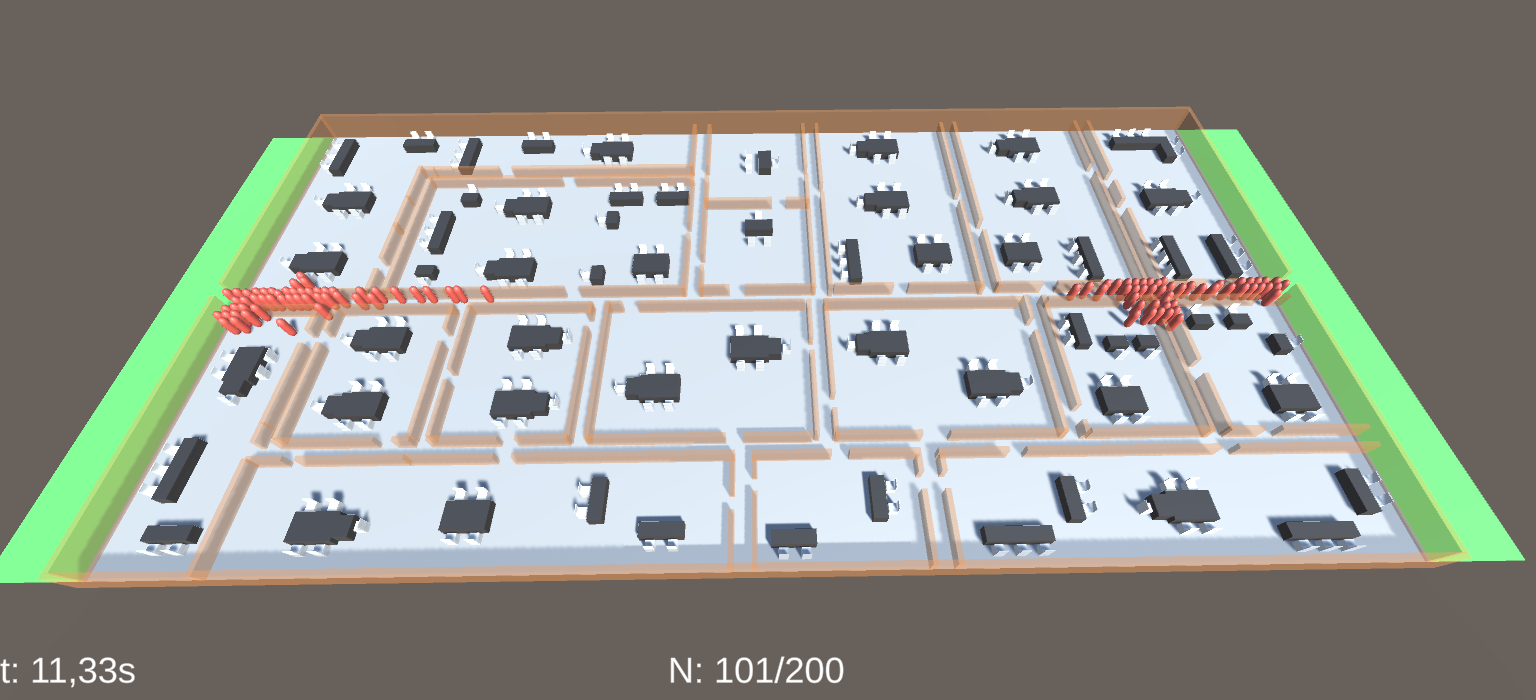
\includegraphics[scale=0.17]{1.(b) Couloir autre 80cm - Observations.png}\newline
\newline
$\hspace*{0.2cm}$- La circulation est relativement fluide, dans le couloir principal aucun problème car il est de 1m (1.a) et dans les autres couloirs comme ils sont plus petits, cela permet d'avoir moins de personnes qui essaye de rentrer en même temps dans
le couloir principal. De ce fait, le temps pourra peut-être être amoindri.
\newline
$\hspace*{0.2cm}$- Le temps moyen est moindre que celui pour des couloirs de 1m donc l'hypothèse est réfuté. Et pour autant on peut pas en deduire qu'il faille des couloirs plus petit car l'expérience avec 1m25 prouve le contraire.
\newline\newline


1.(b) Couloir Autre 1m :
\newline\newline
Temps moyen de dernière sortie : 23.20 s
\newline
$\hspace*{0.2cm}$-Malgre une fluidité dans les couloirs et leur changement du à une taille égales de ces derniers, les temps sont plus importants que pour d'autre simulation.
\newline\newline

1.(b) Couloir Autre 1m25 :
\newline\newline
Temps moyen de dernière sortie : 21.27 s
\newline
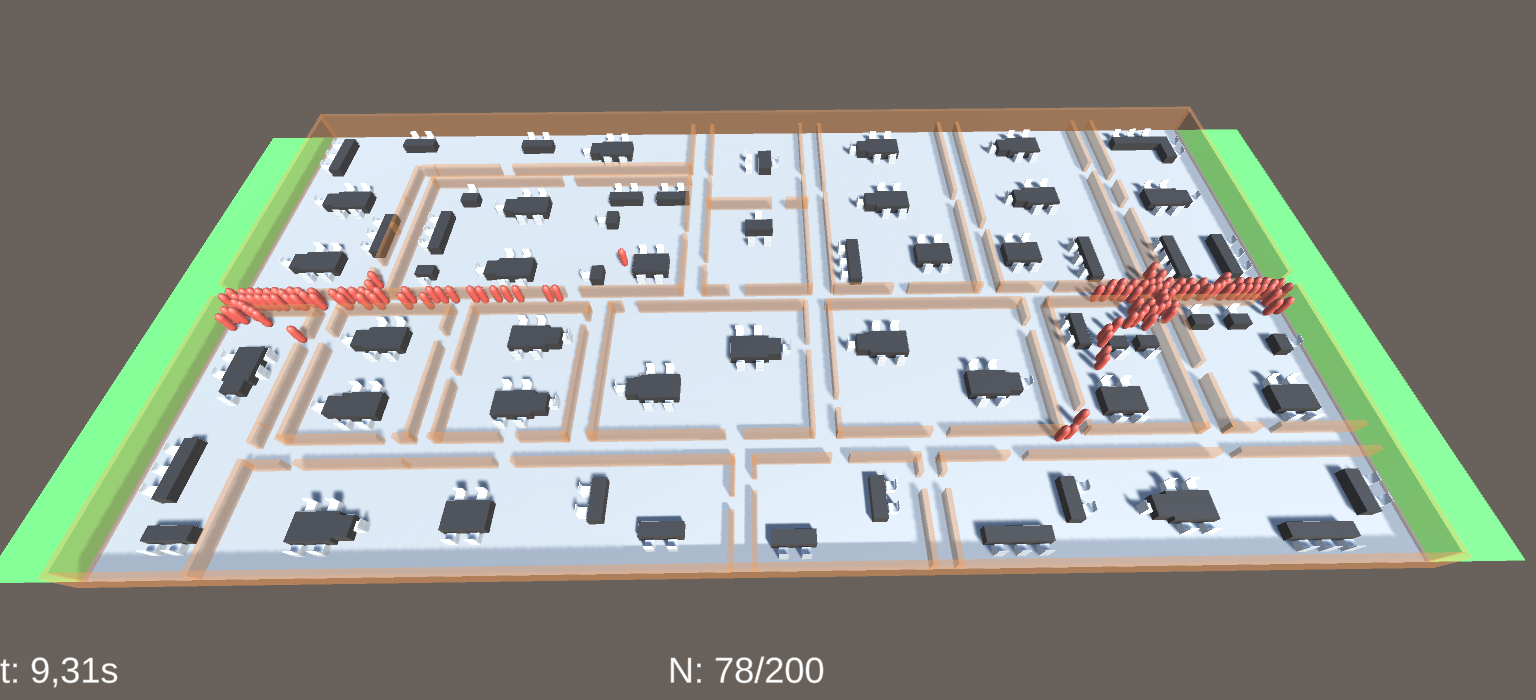
\includegraphics[scale=0.17]{1.(b) Couloir Autre 1m25 - Observations.png}\newline
\newline
$\hspace*{0.2cm}$- La largeur des autres couloirs permet un accès facile au couloir principal ce qui peux expliquer le gain de temps.
\newline
$\hspace*{0.2cm}$- Il sera nécessaire de comprendre si il vaut mieux des plus larges couloirs ou plus fin (ici le temps est meilleur pour 1m25 que pour 80cm et 1m50)
\newline\newline

1.(b) Couloir Autre 1m50 :
\newline\newline
Temps moyen de dernière sortie : 22.54 s
\newline
$\hspace*{0.2cm}$-Il peut y avoir 3 personnes dans les couloirs de 1m50, donc quand il arrive vers le couloir principal, il y a des bousculades pour y rentrer, on a un effet entonnoir qui se fait sentir.
\newline
$\hspace*{0.2cm}$-De plus, la taille des bureaux rétrécis comme la taille des couloirs augmentent, donc les circulations dans les bureaux deviennent de plus en plus difficile.
\newline
$\hspace*{0.2cm}$- Donc comme cela était prévisible, il ne suffit pas d'avoir d'immense couloir autre que le principal pour réduire le temps.
\newline\newline

1.(b) Couloir Autre 2m :
\newline\newline
Temps moyen de dernière sortie : 22.08s
\newline
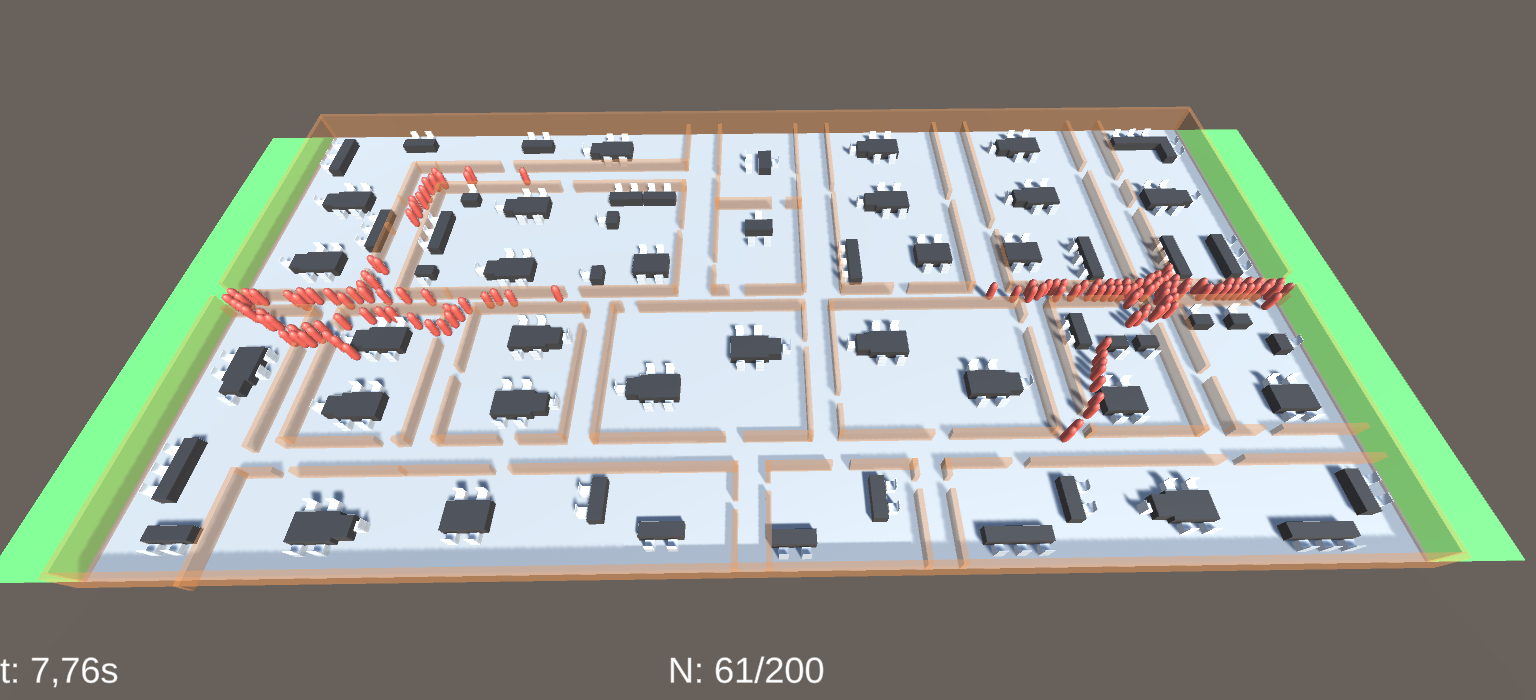
\includegraphics[scale=0.17]{1.(b) Couloir Autre 2m - Observations.png}\newline
\newline
$\hspace*{0.2cm}$- Comme les autres couloirs sont très grand, on a d'important flux qui arrivent dans les couloirs principaux ce qui génère de nombreuses bousculades.
\newline\newline

\section{Couloir taille unique}

1.(b) Couloirs 80cm :
\newline\newline
Temps moyen de dernière sortie : 28.70s
\newline
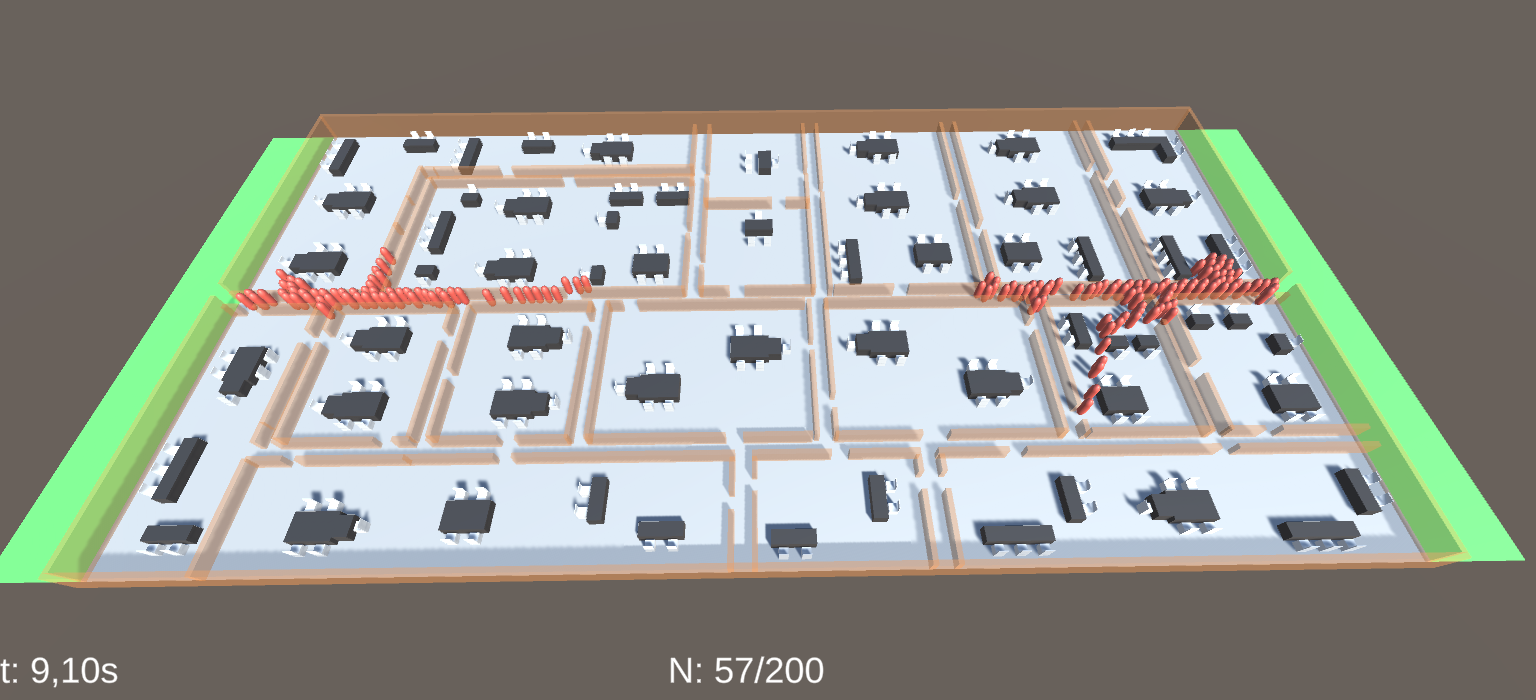
\includegraphics[scale=0.17]{1.(b) Couloirs 80cm -Observations.png}\newline
\newline
$\hspace*{0.2cm}$- Les embouteillages près des portes de sorties sont intensifiés à cause des petits couloirs.
\newline
$\hspace*{0.2cm}$- De plus parfois il y a seulement une personne qui passe en largeur dans le couloir principal.
\newline\newline

1.(b) Couloirs 1m :
\newline\newline
Temps moyen de dernière sortie : 24.51 s
\newline\newline

1.(b) Couloirs 1m25 :
\newline\newline
Temps moyen de dernière sortie : 20.42s
\newline
$\hspace*{0.2cm}$- La sortie est fluide malgrès quelque blocage au niveau des portes de sorties et de certaines intersections (comme dans chaque simulation). Mais comme 1m25 est relativement proche de 1m,
les personnes arrivent à passer fluidement au niveau des portes.
\newline
$\hspace*{0.2cm}$-Il y a plus de fluidité dans les carrefours comme ils sont plus larges.
\newline\newline

1.(b) Couloirs 1m50 :
\newline\newline
Temps moyen de dernière sortie : 24.62s
\newline
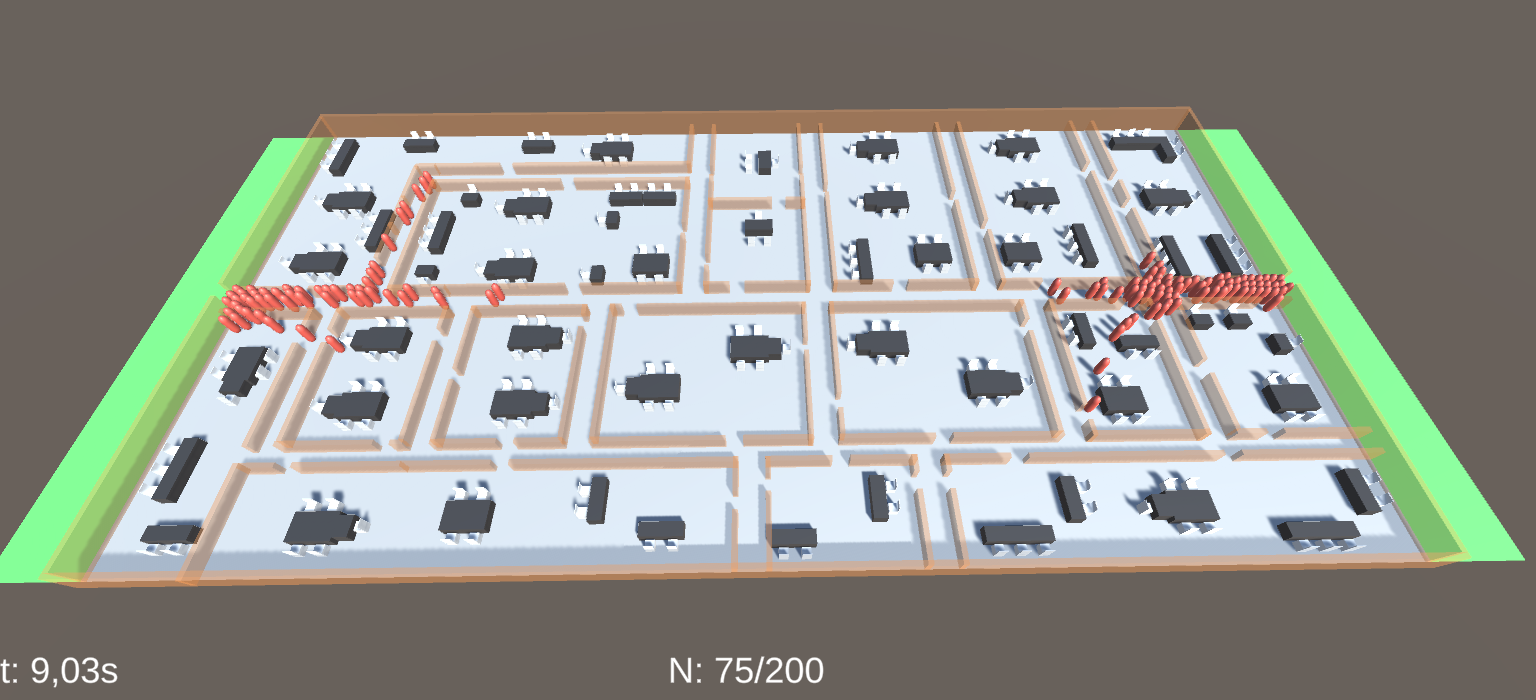
\includegraphics[scale=0.17]{1.(b) Couloirs 1m50- Problème.png}\newline
\newline
$\hspace*{0.2cm}$-Comme la porte est trop petit par rapport aux couloirs y menant, il y a un gros blocage au niveau des portes de sorties.
\newline\newline

1.(b) Couloirs 2m :
\newline\newline
Temps moyen de dernière sortie : 24.51s
\newline
$\hspace*{0.2cm}$- Il y a des très gros flux ce qui créer des blocages au niveau des portes.
\newline\newline

\underline{Résultat : Couloirs Autre }
\newline
Contrairement à ce que je pensais il ne suffit pas d'avoir tous les couloirs de la même taille que le couloir principal pour avoir le meilleur temps.
Il est aussi nécessaire d'avoir parfois de grands couloirs menant au couloir principaux pour augmenter le flux dans les couloirs principaux. (Ceci sans effet entonnoir car
le flux arrive en entier dans le couloir car c'est sous forme de T)
\newline
Ci-dessous le graphe des resultats, on voit que le meilleur temps est quand les autres couloirs sont de 1m25.
\newline
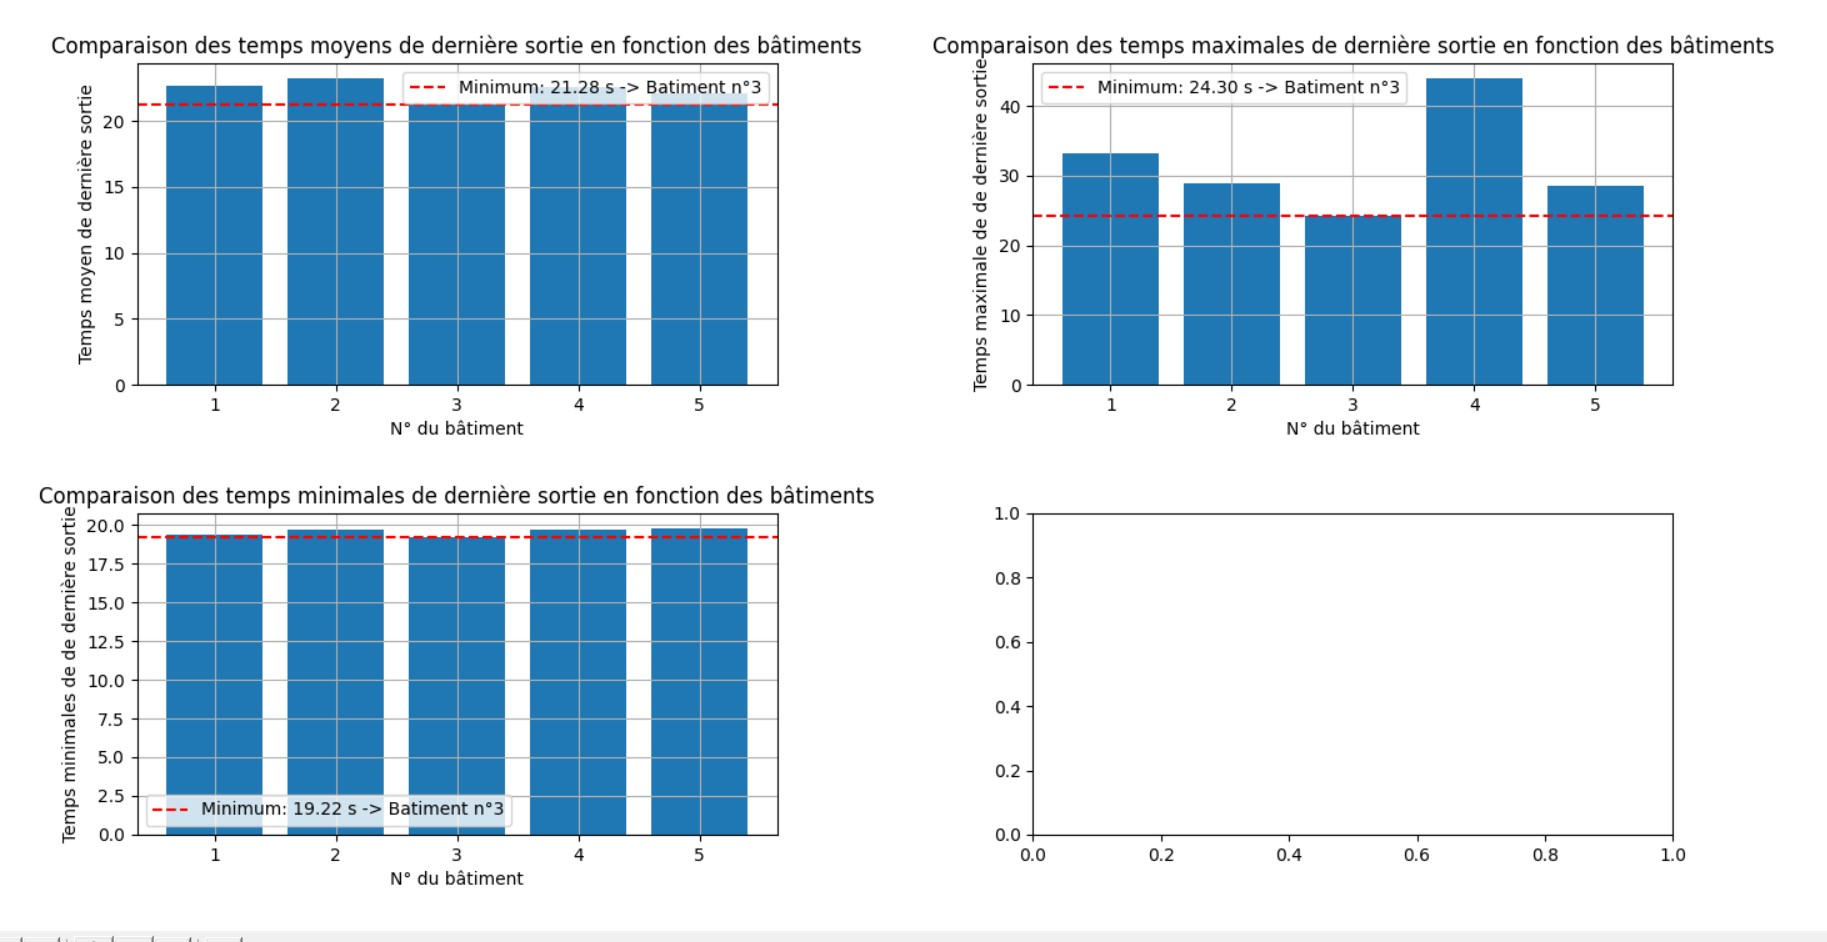
\includegraphics[scale=0.4]{1.(b) Resultat.jpg}\newline
\newline\newline

\underline{Résultat : Couloirs}
\newline
Le meilleur temps est obtenu quand tous les couloirs sont de 1m25 (cela valide qu'il faut que les couloirs soient de taille unique)
\newline
Cependant Contrairement à ce que j'attendais il vaut mieux avoir des couloirs un peu plus grand que les portes de sorties car cela permet d'avoir de plus gros flux
dans les couloirs principaux et l'embouteillage devant les portes est négligeable car les couloirs sont pas trop grand par rapport à la porte de sortie.
\newline
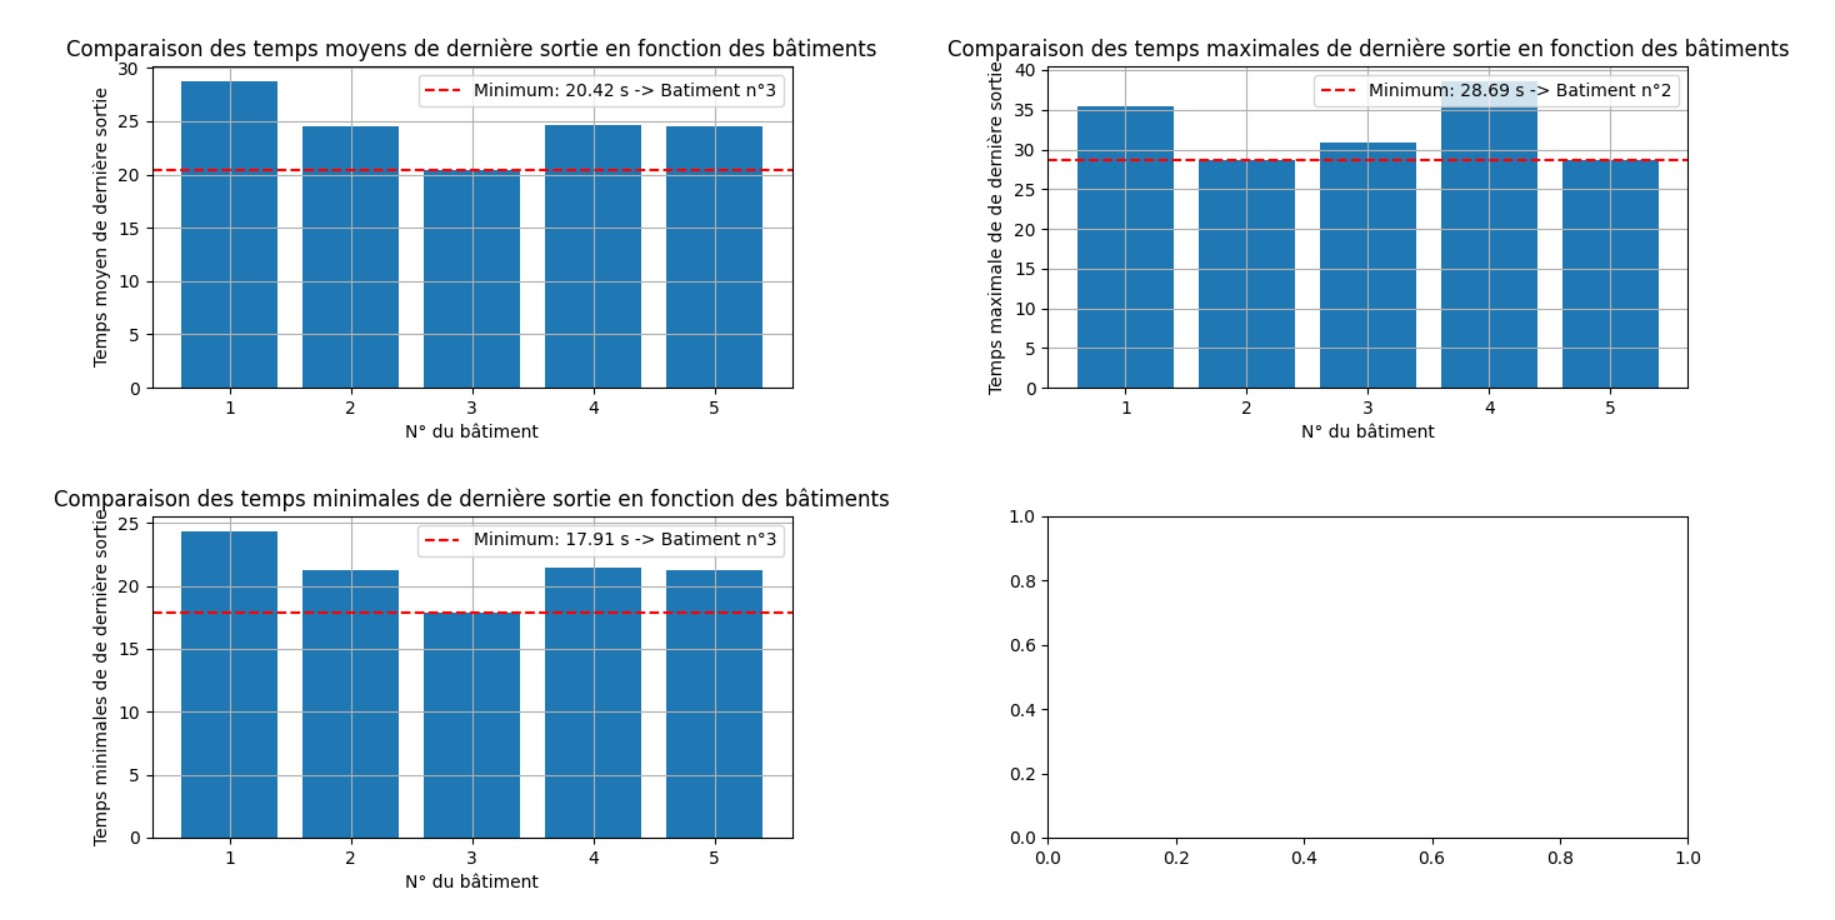
\includegraphics[scale=0.4]{1.(b) Resultat-bis.jpg}\newline
\newline\newline

\underline{Résultat Finaux :}
\newline
Finalement on vient de voir que la taille des couloirs influe sur le temps de sortie. Pour faire en sorte d'avoir un temps minimal, il faut que les couloirs soit un peu plus large que la sortie
ainsi on a pas enormement plus de blocage au niveau des portes et en même temps le flux est plus important car le couloir est un peu plus large.
1m25 pour tous les couloirs est le meilleur que l'on est trouvé.
\newline
Au final le 1.(a) ne sert pas à grand chose du coup.
\newline\newline
L'hypothèse gardé est : La taille des couloirs doit être unique(car mieux quand tout fait 1m25 que tous les autres) et un peu plus grande que celle des portes de sorties principales.

\end{document}